\part{Soluções Apresentadas}
\chapter[Introdução]{Introdução}
Neste capítulo abordaremos todas as soluções idealizadas para o projeto. O capítulo está dividido conforme os grupos descritos na subseção ~\ref{subsec:divisao}.

\chapter[Estruturas e Materiais]{Estruturas e Materiais}

\chapter[Smart Grid]{Smart Grid}

\begin{table}[h]
  \centering
  \caption{Energia Eólica - Vantagens x Desvantagens}
  \label{my-label}
  \begin{tabular}{|l|l|}
    \hline
    \multicolumn{2}{|c|}{\textbf{Energia Eólica}}                                         \\ \hline
    \multicolumn{1}{|c|}{\textbf{Vantagens}} & \multicolumn{1}{c|}{\textbf{Desvantagens}} \\ \hline
    Energia Sustentável                      & Alto Custo                                 \\ \hline
    Energia Limpa                            & Baixa velocidade do vento na região        \\ \hline
    Energia Renovável                        & Pouca Área para instalação dos equipamento \\ \hline
  \end{tabular}
\end{table}

\begin{table}[h]
  \centering
  \caption{Energia Solar Fotovoltaica - Vantagens x Desvantagens}
  \label{my-label}
  \begin{tabular}{|l|c|}
    \hline
    \multicolumn{2}{|c|}{\textbf{Energia Solar Fotovoltaica}}                                                \\ \hline
    \multicolumn{1}{|c|}{\textbf{Vantagens}}             & \textbf{Desvantagens}                             \\ \hline
    Energia Sustentável                                  & \multicolumn{1}{l|}{Alto custo financeiro}        \\ \hline
    Energia limpa                                        & \multicolumn{1}{l|}{Geração apenas durante o dia} \\ \hline
    Simples manutenção                                   & -                                                 \\ \hline
    Alta incidência solar na região                      & -                                                 \\ \hline
    Vida útil dos painéis longa                          & -                                                 \\ \hline
    Tempo de retorno do investimento em cerca de 10 anos & -                                                 \\ \hline
  \end{tabular}
\end{table}


\begin{table}[h]
  \centering
  \caption{Gerador Movido a Biodiesel - Vantagens x Desvantagens}
  \label{my-label}
  \begin{tabular}{|c|l|}
    \hline
    \multicolumn{2}{|c|}{\textbf{Gerador Movido a Biodiesel}}                                            \\ \hline
    \textbf{Vantagens}                                      & \multicolumn{1}{c|}{\textbf{Desvantagens}} \\ \hline
    \multicolumn{1}{|l|}{Energia Sustentável}               & Alto consumo de biodiesel                  \\ \hline
    \multicolumn{1}{|l|}{Biocombustível produzido pela FGA} & Rendimento baixo                           \\ \hline
    -                                                       & Alto custo financeiro                      \\ \hline
    -                                                       & Manutenção periódica                       \\ \hline
  \end{tabular}
\end{table}


\chapter[Controle de Acesso]{Controle de Acesso}
\section{Escolha da Tecnologia}
A área de Controle de Acesso está aqui subdividida em três grandes principais frentes tecnológicas.
São elas: controle da entrada do estacionamento privativo, controle da entrada em salas e laboratórios
e, por fim, controle de frequência durante as aulas.

Dentre essas frentes, foram elegidas três possibilidades diferentes para a inserção na Universidade.
A tabela a seguir elicita-as, bem como apresenta as vantagens e desvantagens para cada um dos casos.

\begin{table}[h]
  \centering
  \caption{Tecnologias de Controle de Acesso - Vantagens x Desvantagens}
  \label{my-label}
  \begin{tabular}{|l|l|l|}
    \hline
    \multicolumn{1}{|c|}{\textbf{Tecnologia}} & \multicolumn{1}{c|}{\textbf{Vantagens}}                                                                         & \multicolumn{1}{c|}{\textbf{Desvantagens}}                                                                                                            \\ \hline
    Leitor biométrico                         & \begin{tabular}[c]{@{}l@{}}- Difícil de burlar \\ - Confiável\end{tabular}                                      & \begin{tabular}[c]{@{}l@{}}- Pode gerar falhas na leitura \\ - Não reconhecer uma \\ digital cadastrada\\ - Sistema caro\\ - Sistema frágil\end{tabular} \\ \hline
    Leitor facial/ Leitor de íris             & \begin{tabular}[c]{@{}l@{}}- Difícil de burlar \\ - Confiável\end{tabular}                                      & \begin{tabular}[c]{@{}l@{}}- Sistema de implementação\\ cara\\ - Demora para análise de \\cada pessoa\\ - Risco de furto\\ - Frágil\end{tabular}          \\ \hline
    Leitor RFID                               & \begin{tabular}[c]{@{}l@{}}- Fácil de utilizar\\ - Difícil de burlar\\ - Único para cada estudante\end{tabular} & \begin{tabular}[c]{@{}l@{}}- Custo extra para a \\faculdade\\ - Risco de perda do \\documento\end{tabular}                                                \\ \hline
  \end{tabular}
\end{table}

Apesar de todas as tecnologias sugeridas apresentarem vantagens e desvantagens, o sistema RFID foi o escolhido para atender
a demanda. Esta escolha se deu em virtude deste ser mais eficaz, eficiente e mais acessível financeiramente em relação aos
outros.

\subsection{Breve Descrição da Tecnologia RFID}
O sistema funciona RFID (do inglês \textit{Radio-Frequency IDentification}) é um tecnologia que permite identificação automática
 através de sinais de rádio. Neste projeto será implementado de  por meio de um chip dentro de um cartão, armazenando o
 nome e matrícula do aluno dono do documento e sempre que o documento for apresentado, seus dados serão apresentados nos
 display dos equipamentos. Levando em conta que tanto alunos como professores serão portadores deste documento com chip,
 para o alunos o cartão será utilizado como carteirinha, e para os professores como crachá.

Apesar de todo o grupo de controle de acesso utilizar esta ferramenta, cada uma das frentes utiliza o sistema de forma
diferente e com aparelhos diferentes. Desta forma, cada área tem suas particularidades de funcionamento e regras, como será
 mostrado e explicado a seguir.

\section{Controle de Frequência}
Para o controle de frequência nas aulas, será utilizado o seguinte aparelho (apresentado anteriormente no Ponto de Controle 1).
O funcionamento dele acontece independente de sinal de WiFi e o aparelho é de porte único do professor.

\begin{figure}[!h]
  \centering
  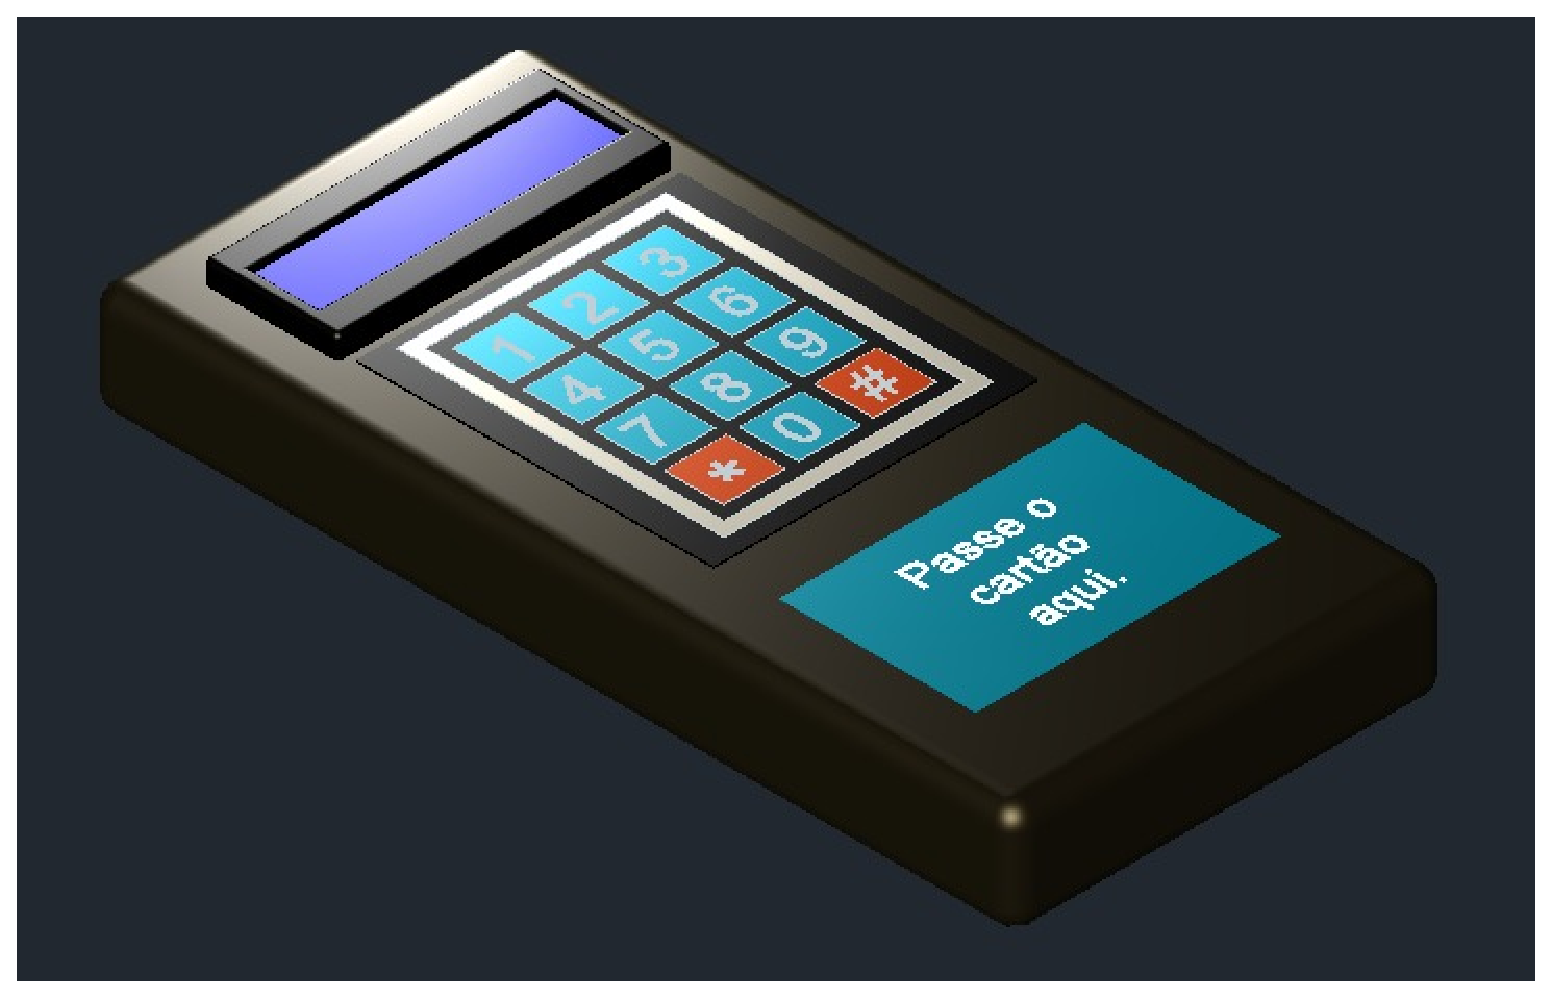
\includegraphics[keepaspectratio=true,scale=0.45]{figuras/freq.eps}
  \caption{Aparelho Para Controle de Frequência}
\end{figure}

Em relação à aspectos técnicos do aparelho, a figura a seguir mostra detalhadamente quais os instrumentos utilizados.

\begin{figure}[h]
  \centering
  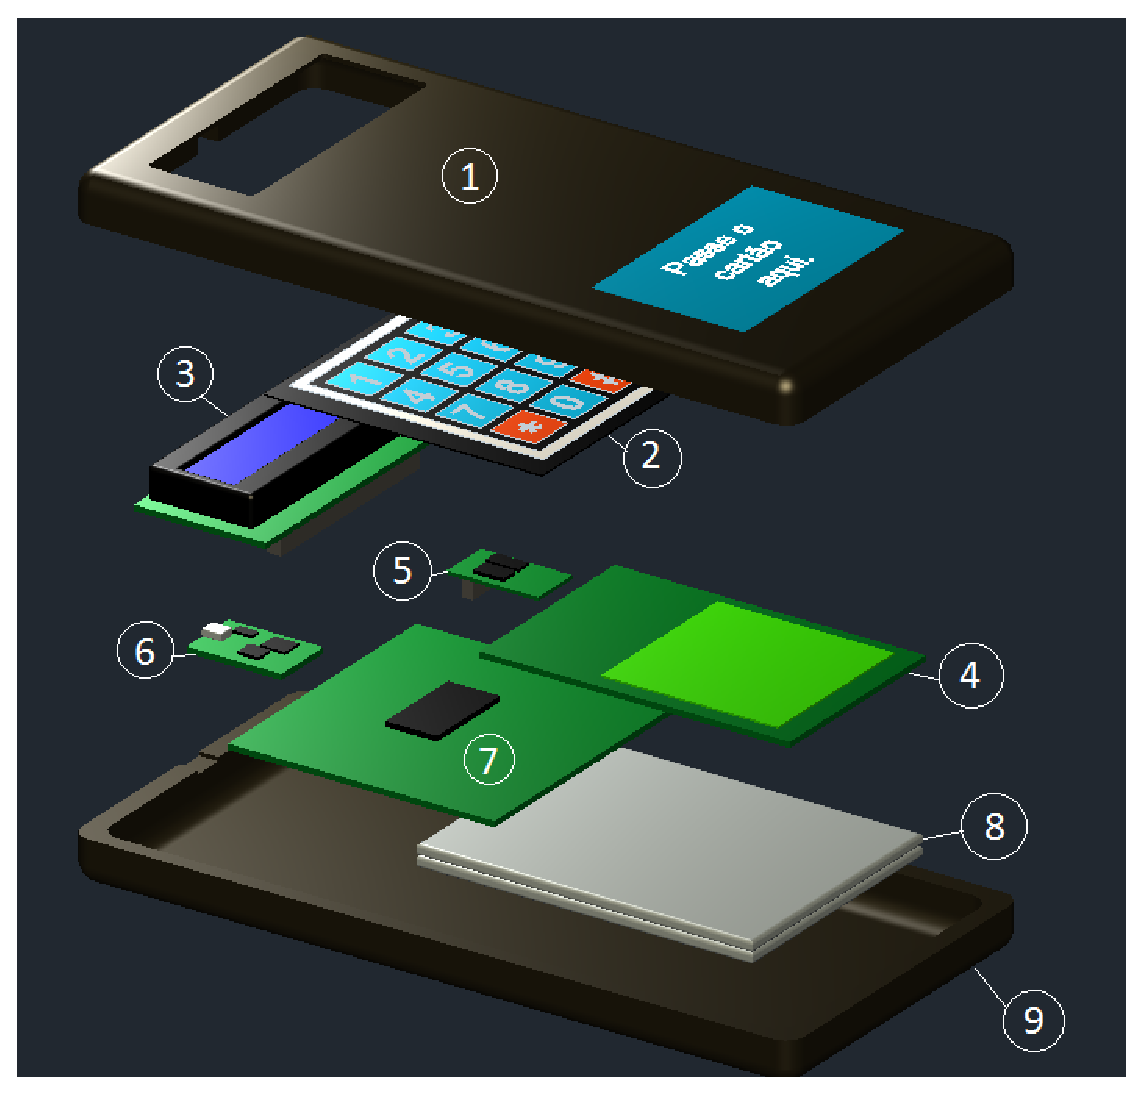
\includegraphics[keepaspectratio=true,scale=0.45]{figuras/aberto.eps}
  \caption{Aparelho Para Controle de Frequência Detalhado}
\end{figure}

Cada um dos componentes possui sua função individual:
\begin{itemize}
  \item Componentes 1 e 9: Case superior e inferior. Há um orifício na parte superior do dispositivo para passagem do conector USB.
  \item Componente 2: Teclado matricial de película 12 teclas.
  \item Componente 3: Display LCD 16x2 com backlight
  \item Componente 4: módulo Leitor de cartões RFID Mfrc522 Mifare, faz leitura e escrita em cartões RFID.
  \item Componente 5: Módulo WiFi ESP8266 ESP-01, se conecta com a rede wifi e transmite e recebe dados servidor online.
  \item Componente 6: Módulo Carregador de Baterias de Lítio TP4056, carrega a bateria através do seu conector USB.
  \item Componente 7: Placa controladora faz as conexões com os demais componentes e possui um microcontrolador ATmega1280 16au da família AVR com o bootloader do Arduino mega.
  \item Componente 8: Baterias do tablet Dl Lenoxx Navcity Phaser. Possuem capacidade de 2000mAh e tensão de 3,7v.
\end{itemize}



\chapter[Instrumentação e Controle]{Instrumentação e Controle}

\chapter[Interfaces e Processamento de Software]{Interfaces e Processamento de Software}
